\documentclass[compress,10pt,aspectratio=169]{beamer}
%\setbeamertemplate{background canvas}[bottom=white,top=structure.fg!25]
%\usetheme{Hannover}
\setbeamertemplate{headline}{}
\setbeamertemplate{footline}{June 27, 2020 - SDRA}
\setbeamersize{text margin left=0cm}
\usepackage{appendixnumberbeamer}
\usepackage{hyperref,listings,picinpar,mathtools} % ,enumitem}
\usepackage{color}
\usepackage{tabularx}
\settowidth{\leftmargini}{\usebeamertemplate{itemize item}}
\addtolength{\leftmargini}{\labelsep}

\definecolor{grey}{rgb}{0.95,0.95,0.95}
\definecolor{red}{rgb}{1.0,0.0,0.0}
\definecolor{green}{rgb}{0.0,0.6,0.0}
\definecolor{blue}{rgb}{0.0,0.0,1.0}
\lstloadlanguages{bash,Java,C,C++,csh,make,sh}%%[Visual]Basic,xml}
\lstset{frame=none,basicstyle=\footnotesize,breaklines,tabsize=2,captionpos=b,prebreak={\hbox{$\rightarrow$}},postbreak={\hbox{$\hookrightarrow$}},showstringspaces=false,backgroundcolor=\color{grey}\bfseries,keywordstyle=\color{blue},commentstyle=\color{green}\textit,stringstyle=\color{red}\ttfamily,abovecaptionskip=2pt,aboveskip=0pt,belowskip=0pt,belowcaptionskip=0pt}
%\lstset{moredelim=[is][\color{red}]{_+_}{_+_}}

\beamertemplatefootpagenumber
\beamertemplatenavigationsymbolsempty
\setbeamertemplate{footline}[page number]{}
\setbeamertemplate{page number in head/foot}{}

\usepackage{graphicx,verbatim,multicol,amsmath,bm}

\begin{document}

\begin{frame}[fragile,noframenumbering]\frametitle{LFSR / FPGA stuff}

\begin{minipage}[t]{\linewidth}
\begin{minipage}{.5\linewidth}
Principle:\\
\hspace{1cm}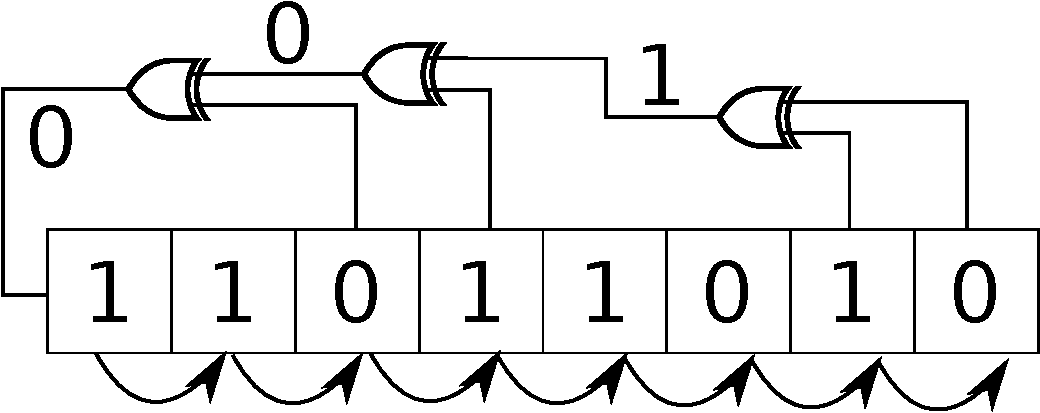
\includegraphics[width=0.7\textwidth]{lfsr_scheme.pdf}

Combinatorial / sequencial concepts\\
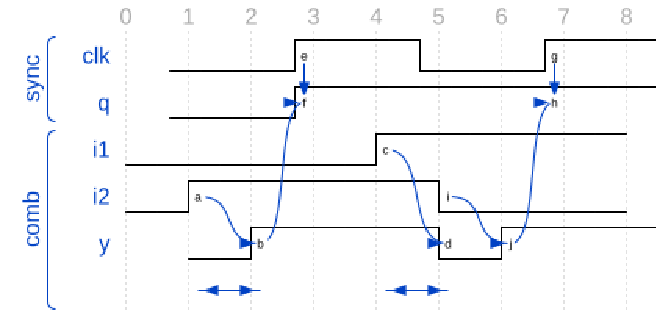
\includegraphics[width=0.9\textwidth]{behav.pdf}
\end{minipage}
\begin{minipage}{.5\linewidth}

Basic Amaranth concept:

{\small
\begin{verbatim}
class MyClass(Elaboratable):

    def elaborate(self, platform):
        m = Module()
        
        cSig = Signal()
        sSig = Signal(2)
        
        m.d.comb += cSig.eq(sSig[1] ^ sSig[0])
        m.d.sync += sSig.eq(Cat(sSig[1], cSig))
        
        return m
\end{verbatim}
}

\end{minipage}
\end{minipage}

\vspace{0.5cm}
\hspace{0.5cm}{\footnotesize
amaranth $\rightarrow$ verilog $\rightarrow$ synthesis (yosys, Vivado, ...)
$\rightarrow$ PnR (nextpnr, vtr, vivado, ...)
$\rightarrow$ bitstream $\rightarrow$ programmer
}
\end{frame}

\begin{frame}[fragile,noframenumbering]\frametitle{LFSR: basic idea}

\begin{minipage}[t]{\linewidth}
\begin{minipage}{.6\linewidth}
\hspace{1cm}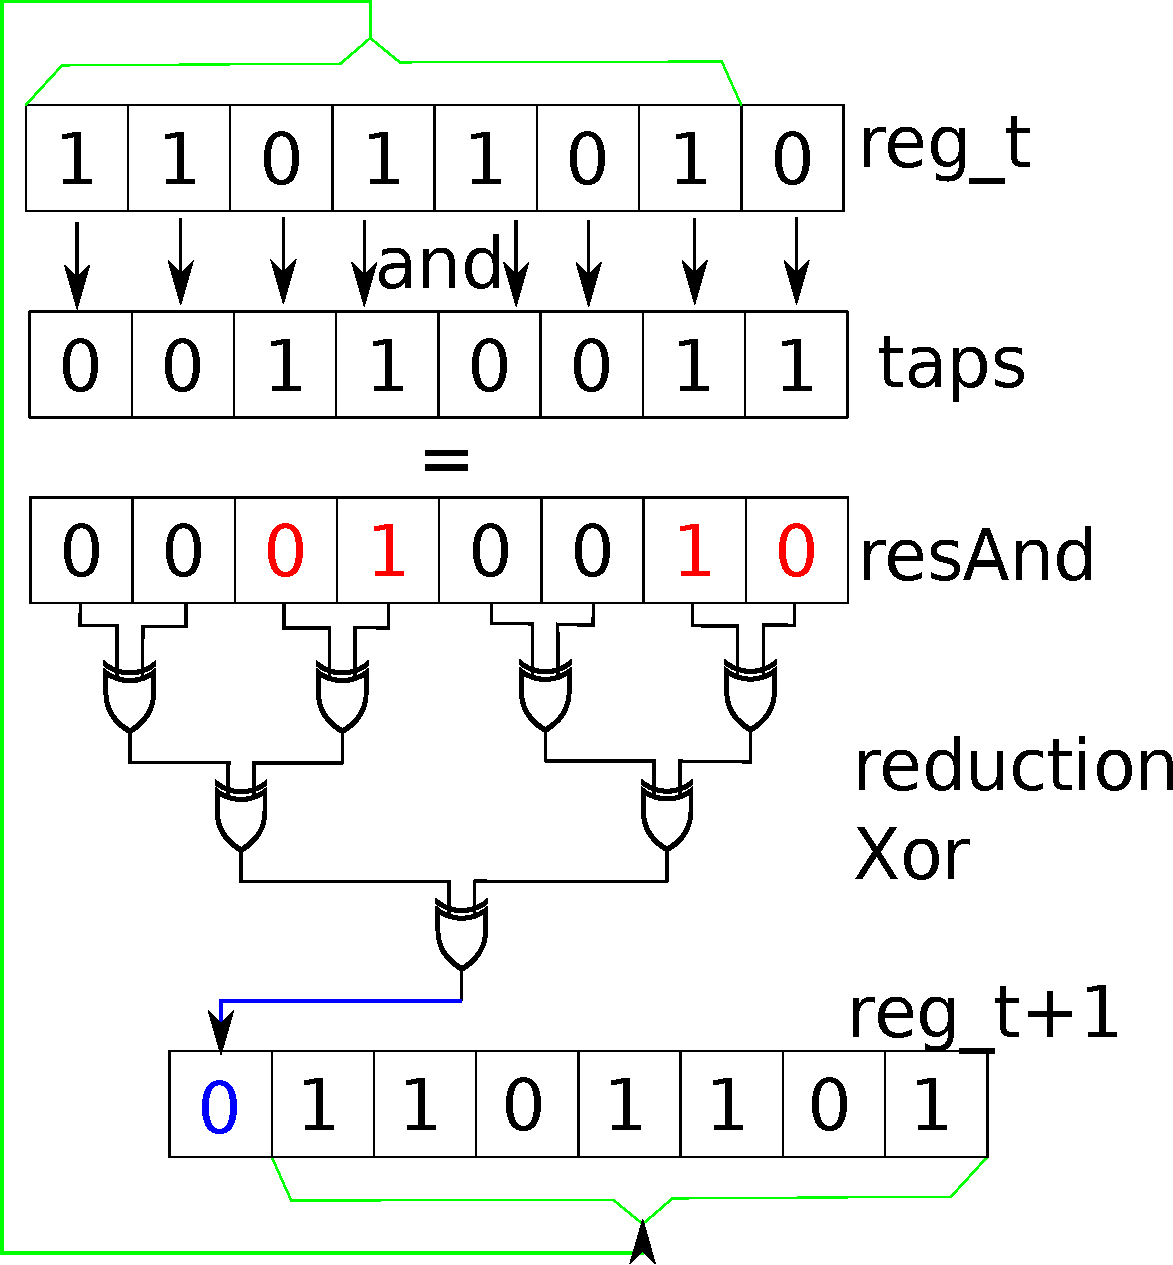
\includegraphics[width=0.7\textwidth]{lfsr_impl.pdf}
\end{minipage}
\begin{minipage}{.4\linewidth}
{\tt AND} truth table:

\begin{tabular}{c|c|c|}
i1\verb^\^i2 & 0 & 1 \\
\hline
0 & 0 & 0 \\ 
\hline
1 & 0 & 1 \\ 
\hline
\end{tabular}

TAPs with AND: mask ($y_n = i1_n \& i2_n$)

\vspace{1cm}
{\tt XOR} truth table:

\begin{tabular}{c|c|c|}
i1\verb^\^i2 & 0 & 1 \\
\hline
0 & 0 & 1 \\ 
\hline
1 & 1 & 0 \\ 
\hline
\end{tabular}

reduction Xor: ($y = i_{0} \oplus i_1 \oplus i_2 \oplus ... \oplus i_{n-1}$)
\end{minipage}
\end{minipage}

With taps set at synthesis time $\rightarrow$ gateware is optimize (no more AND,
picks relevant bits and improve the LUT's truth table).

\end{frame}
\begin{frame}\frametitle{NCO}
\center
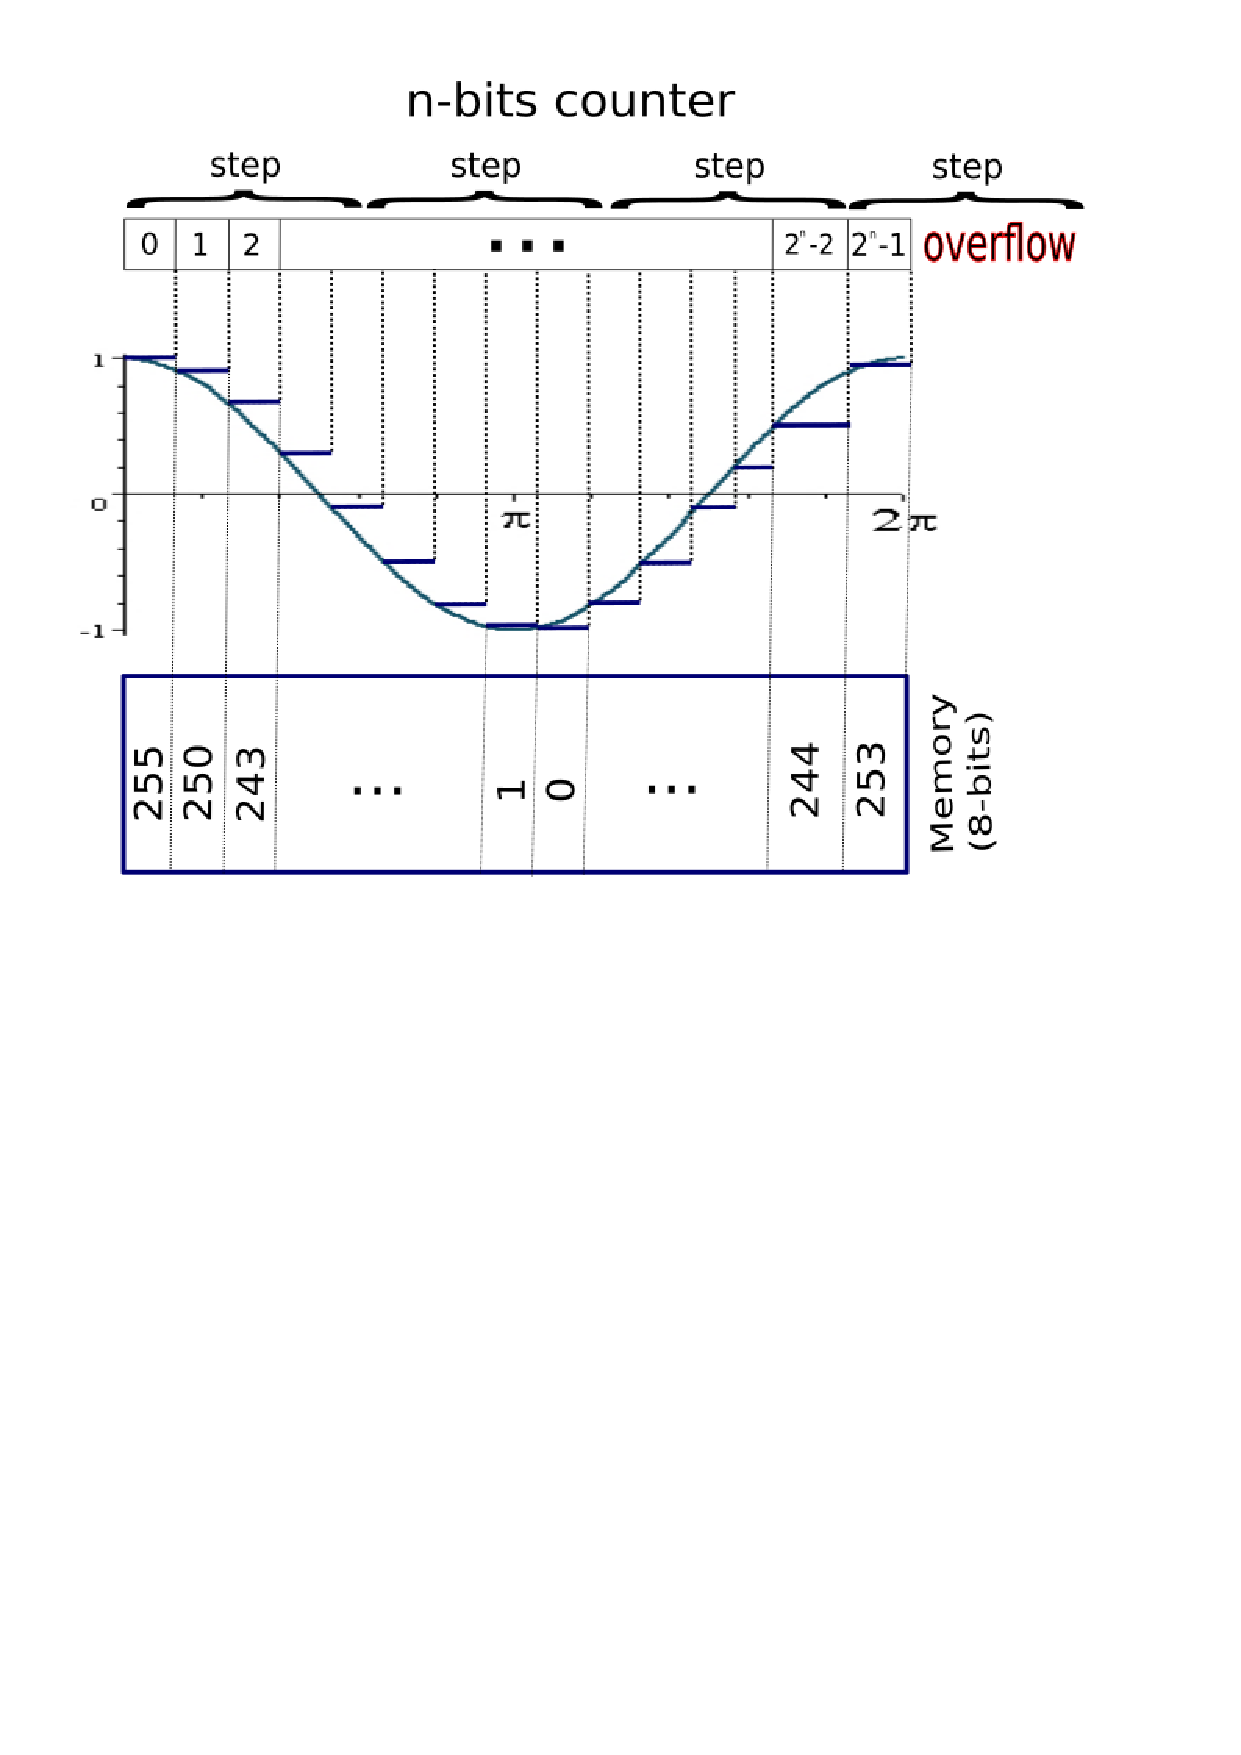
\includegraphics[width=0.7\textwidth]{./NCOOO.pdf}
\end{frame}

\begin{frame}[fragile,noframenumbering]\frametitle{hardware aspects}

Amaranth gatewares are (more or less) hardware independant\\
$\Rightarrow$ a platform description is required

see: \url{https://github.com/amaranth-lang/amaranth-boards}

\begin{minipage}[t]{\linewidth}
\begin{minipage}{.5\linewidth}
Platform used for development: \\
{\tt Zedboard} ({\tt Xilinx Zynq 7020}) with:
{\footnotesize
\begin{verbatim}
ZedBoardPlatform().build(MyRadioEmitter(),
                         do_program=True)
\end{verbatim}
}

Moving to {\tt radiona ULX3S}:
{\footnotesize
\begin{verbatim}
ULX3S_85F_Platform().build(MyRadioEmitter(),
                           do_program=True)
\end{verbatim}
}

Requires to adapt/change the PLL instance:
{\footnotesize
\begin{verbatim}
def elaboratable(self, platform):
    [...]
    if type(platform) == ZedBoardPlatform:
        # Xilinx PLL/MMCM
    else: # ULX3S
        # Lattice ECP5 PLL
\end{verbatim}
}
\end{minipage}
\begin{minipage}{.5\linewidth}
\center
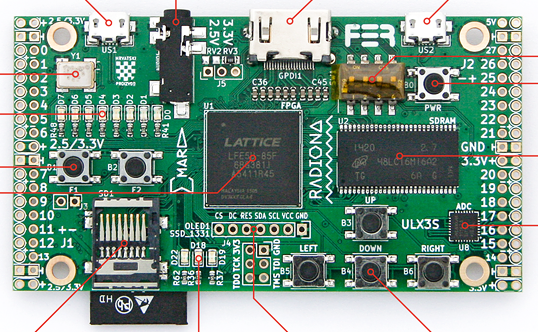
\includegraphics[width=0.7\textwidth]{./ulx3s-legend.png}\\
@source: radiona
\end{minipage}
\end{minipage}

\end{frame}
\end{document}
